\section{Linking induced senses to resources}

\begin{frame}{ Linking induced senses to resources }
	
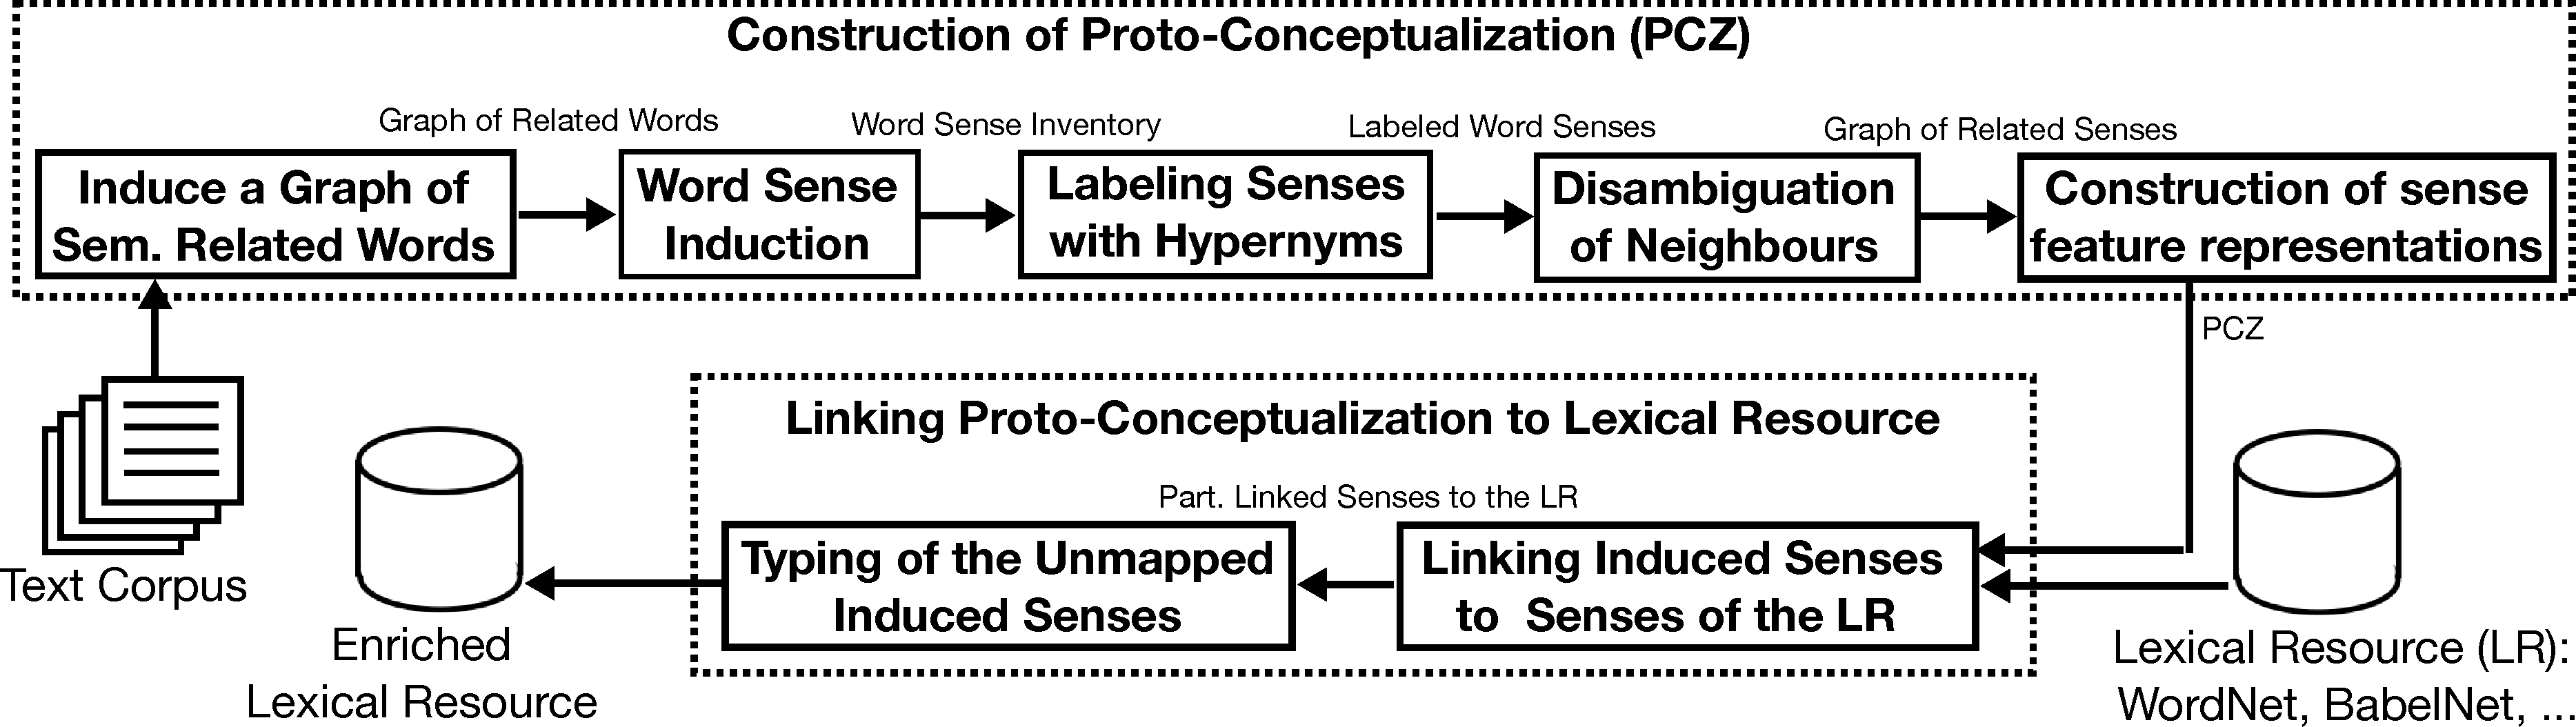
\includegraphics[width=1.05\textwidth]{figures/linking-outline}
\vspace{2em}

\textbf{LREC'16}~\cite{panchenko2016best}, \textbf{ISWC'16}~\cite{faralli2016linked}, \textbf{SENSE@EACL'17}~\cite{panchenko-EtAl:2017:SENSE2017}, \textbf{NLE'18}~\cite{biemann2018framework}

\end{frame}

\begin{frame}{ Linking induced senses to resources }
\vspace{-1em}
%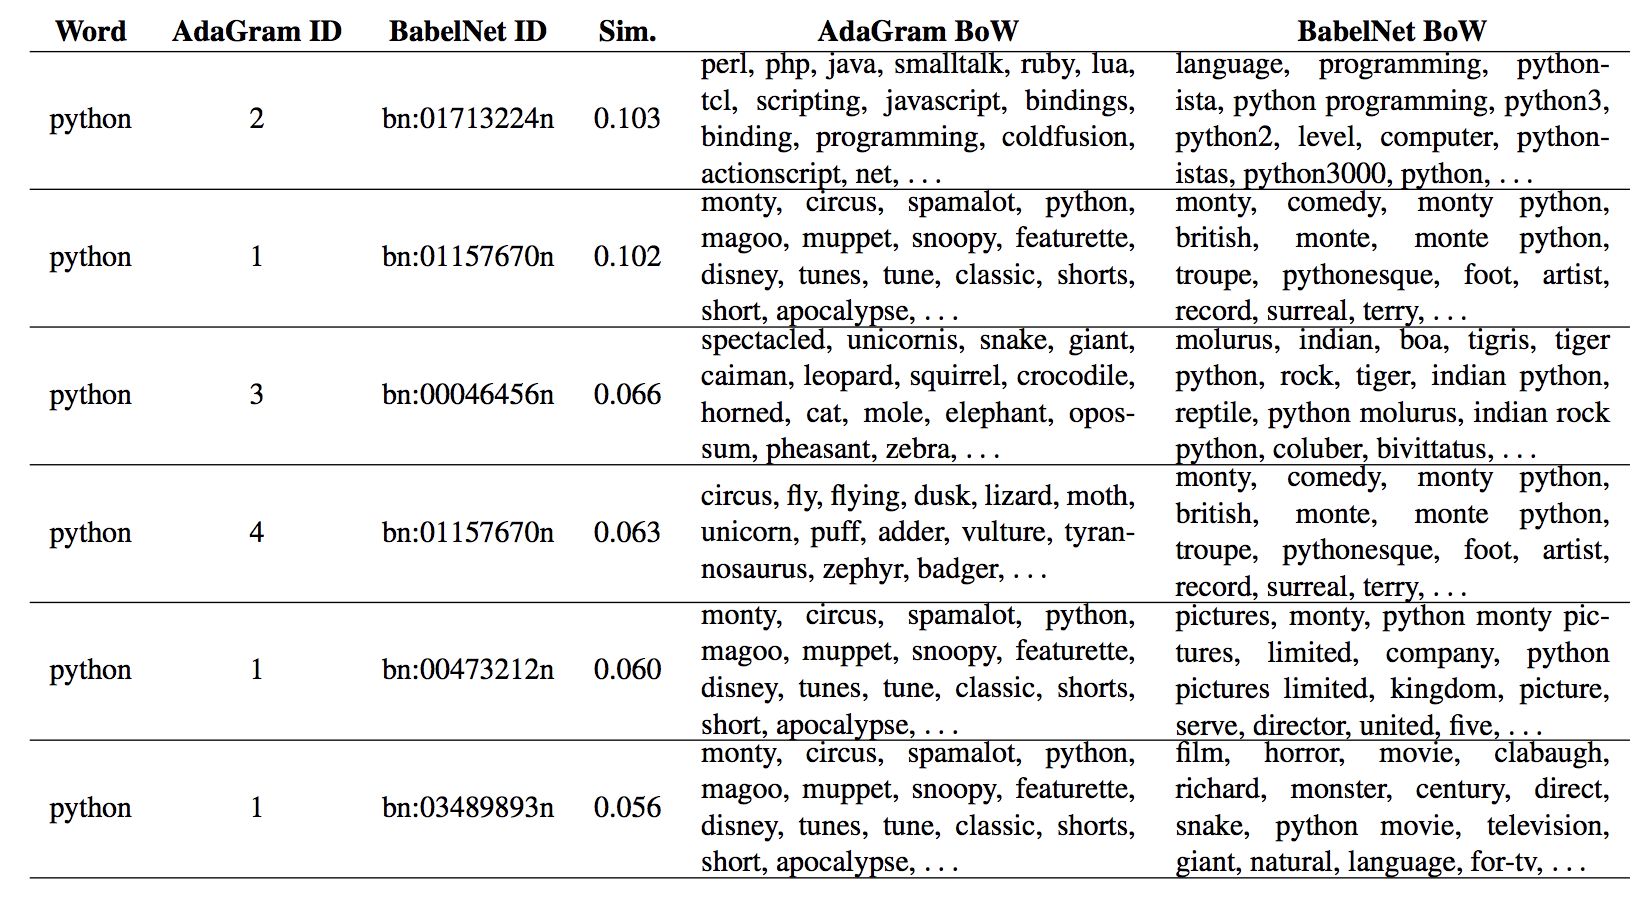
\includegraphics[width=1.05\textwidth]{figures/mapping}
\begin{table}

\tiny  
\begin{center}
\begin{tabular}{ccc p{3cm} p{3cm}}

\bf Word & \bf AdaGram & \bf BabelNet & \bf AdaGram BoW & \bf BabelNet BoW  \\
\hline

python & 2 & bn:01713224n   & perl, php, java, smalltalk, ruby, lua, tcl, scripting, javascript, bindings, binding, programming, coldfusion, actionscript, net, $\ldots$ &  language, programming, pythonista,  python programming, python3, python2, level, computer, pythonistas, python3000, \\ \hline

python & 1 & bn:01157670n & monty, circus, spamalot, python, magoo, muppet, snoopy, featurette, disney, tunes, tune, classic, shorts, short, apocalypse, $\ldots$ &  monty, comedy, monty python, british, monte, monte python, troupe, pythonesque, foot, artist, record, surreal, terry, $\ldots$ \\ \hline

python & 3 & bn:00046456n  & spectacled, unicornis, snake, giant, caiman, leopard, squirrel, crocodile, horned, cat, mole, elephant, opossum, pheasant, $\ldots$ &  molurus, indian, boa, tigris, tiger python, rock, tiger, indian python, reptile, python molurus, indian rock python, coluber, $\ldots$ \\ \hline

python & 4 & bn:01157670n & circus, fly, flying, dusk, lizard, moth, unicorn, puff, adder, vulture, tyrannosaurus, zephyr, badger, $\ldots$ & monty, comedy, monty python, british, monte, monte python, troupe, pythonesque, foot, artist, record, surreal, terry, $\ldots$ \\ \hline

python & 1 & bn:00473212n  & monty, circus, spamalot, python, magoo, muppet, snoopy, featurette, disney, tunes, tune, classic, shorts, short, apocalypse, $\ldots$ &  pictures, monty, python monty pictures, limited, company, python pictures limited, kingdom, picture, serve, director, $\ldots$ \\ \hline

python & 1 & bn:03489893n  & monty, circus, spamalot, python, magoo, muppet, snoopy, featurette, disney, tunes, tune, classic, shorts, short, apocalypse, $\ldots$ &  film, horror, movie, clabaugh, richard, monster, century, direct, snake, python movie, television, giant, natural, language, for-tv, $\ldots$ 
\end{tabular}
\end{center}
\end{table}
	
	
\end{frame}


\begin{frame}{Linking induced senses to resources }


\begin{table}
\tiny
\begin{tabular}{l|p{9cm}} 
\bf Model & \bf Representation of the Sense "disk (medium)"  \\ \hline
\textbf{WordNet}  &  memory, device, floppy, disk, hard, disk, disk, computer, science, computing, diskette, fixed, disk, floppy, magnetic, disc, magnetic, disk, hard, disc,      storage, device \\ \\ \hline 
\textbf{WordNet + Linked} & recorder, disk, floppy, console, diskette, handset, desktop, iPhone, iPod, HDTV, kit, RAM, Discs, Blu-ray, computer, GB, microchip, site, cartridge,          printer, tv, VCR, Disc, player, LCD, software, component, camcorder, cellphone, card, monitor, display, burner, Web, stereo, internet, model, iTunes,         turntable, chip, cable, camera, iphone, notebook, device, server, surface, wafer, page, drive, laptop, screen, pc, television, hardware, YouTube, dvr,        DVD, product, folder, VCR, radio, phone, circuitry, partition, megabyte, peripheral, format, machine, tuner, website, merchandise, equipment, gb, discs,      MP3, hard-drive, piece, video, storage device, memory device, microphone, hd, EP, content, soundtrack, webcam, system, blade, graphic, microprocessor,        collection, document, programming, battery, keyboard, HD, handheld, CDs, reel, web, material, hard-disk, ep, chart, debut, configuration, recording,          album, broadcast, download, fixed disk, planet, pda, microfilm, iPod, videotape, text, cylinder, cpu, canvas, label, sampler, workstation, electrode,         magnetic disc, catheter, magnetic disk, Video, mobile, cd, song, modem, mouse, tube, set, ipad, signal, substrate, vinyl, music, clip, pad, audio,            compilation, memory, message, reissue, ram, CD, subsystem, hdd, touchscreen, electronics, demo, shell, sensor, file, shelf, processor, cassette, extra,       mainframe, motherboard, floppy disk, lp, tape, version, kilobyte, pacemaker, browser, Playstation, pager, module, cache, DVD, movie, Windows, cd-rom, e-book, valve, directory, harddrive, smartphone, audiotape, technology, hard disk, show, computing, computer science, Blu-Ray, blu-ray, HDD, HD-DVD,            scanner, hard disc, gadget, booklet, copier, playback, TiVo, controller, filter, DVDs, gigabyte, paper, mp3, CPU, dvd-r, pipe, cd-r, playlist, slot, VHS,     film, videocassette, interface, adapter, database, manual, book, channel, changer, storage \\ 
\end{tabular}

\end{table}

	
\end{frame}


\begin{frame}{ Linking induced senses to resources }
		\vspace{2em}
		Evaluation of linking accuracy:
		\centering
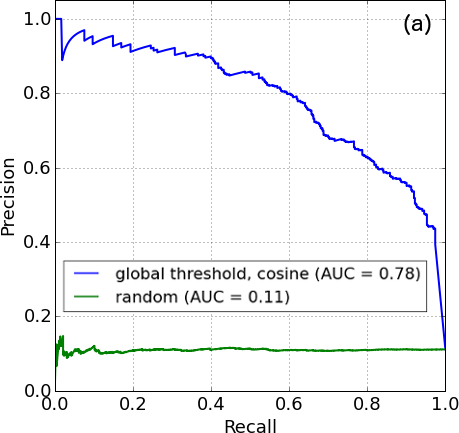
\includegraphics[width=0.41\textwidth]{figures/precision-recall}

\includegraphics[width=0.06\textwidth]{figures/filler}
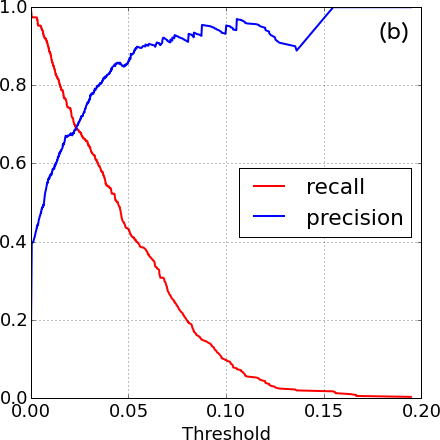
\includegraphics[width=0.40\textwidth]{figures/pr-function-of-threshold}

\end{frame}

\begin{frame}{ Linking induced senses to resources }
\centering
Evaluation of enriched representations based on WSD:

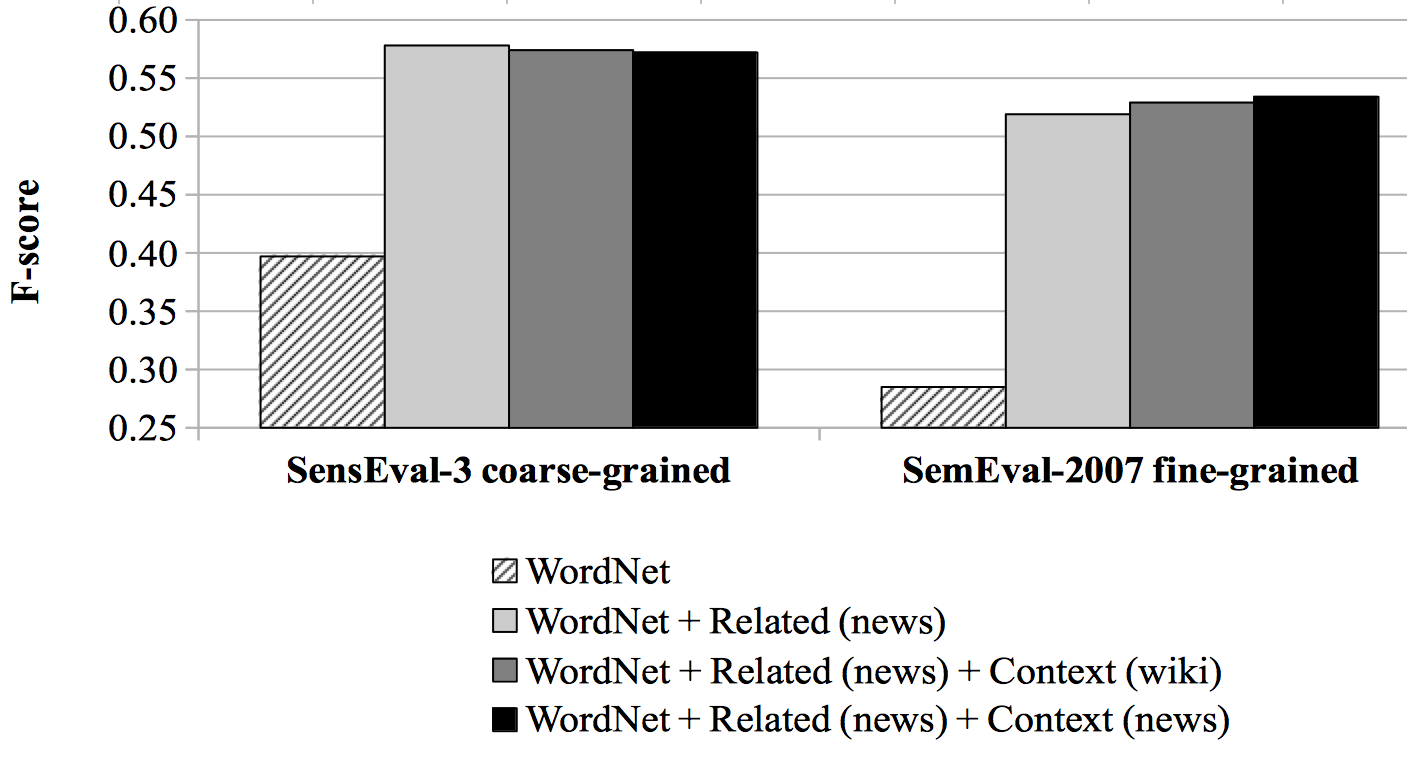
\includegraphics[width=1.0\textwidth]{figures/topic-hist-4}

\end{frame}


